\documentclass[9pt]{article}

\usepackage[a4paper,margin=2cm,top=3cm]{geometry}

% graphics
\usepackage{tikz}
\usepackage{graphicx}

% math
\usepackage{amsmath}
\usepackage{amsfonts}

\usepackage{tabularx}
\usepackage{array}

\usepackage[hidelinks]{hyperref}

% header
\usepackage{fancyhdr}
 
\fancyhf{}
\lhead{دانشگاه صنعتی شریف}
\rhead{تمرینِ نخست}
\chead{مبانیِ برنامه‌نویسی}
\cfoot{\thepage}
 

\usepackage[extrafootnotefeatures]{xepersian}
\settextfont{IRNazanin}


\setlatintextfont[Scale=0.8]{Liberation Serif}
\setdigitfont{IRNazanin}

\begin{document}


%%% first page %%%
	\thispagestyle{empty}
	
	\begin{center}
		به نام خدا
	
		\vskip 80mm
	
		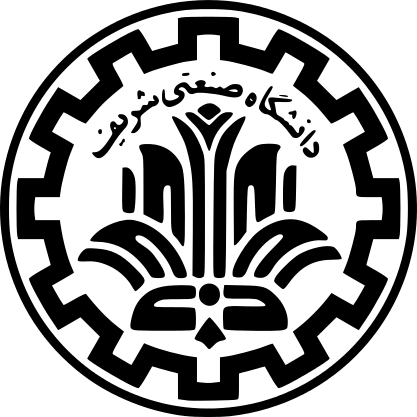
\includegraphics[width=3cm]{sharif-logo}\\
		\huge{درس مبانی برنامه‌سازی} \\
		\bigskip
		\large{نیم‌سال اول 96-97} \\
		\medskip
		دانشکدهٔ مهندسی کامپیوتر\\
		دانشگاه صنعتی شریف \\
		\bigskip
		\hrule
		\medskip
		
		{\def\arraystretch{1.3}
		\begin{tabular}{>{\raggedright}p{0.4\textwidth} >{\raggedleft}p{0.4\textwidth}}
			مدرس & \textbf{مهران ریواده} \tabularnewline
			تمرین & \textbf{نخست} \tabularnewline
			مبحث & \textbf{\rl{IO}} \tabularnewline
			موعد تحویل & \textbf{۱۵ آبان ۱۳۹۶} \tabularnewline

		\end{tabular}}


		\bigskip


	\end{center}
	\begin{large}
	\begin{itemize}
	\item{پاسخ این‌تمرین را در قالب یک‌فایلِ \lr{pdf} در کوئرا آپلود کنید}
	\item{در صورت مشاهده‌ی هرگونه تقلب، نمره‌ی هر دو نفر $-100$ در نظر گرفته خواهد شد.}
	\item{به ازای هر روز دیرکرد در بارگذاری تمرین‌ها، 10 درصد جریمه منظور خواهد شد.}
	\item{در صورت بروز ابهام در مورد سوالات، می‌توانید حداکثر تا 24 ساعت قبل از موعد تحویل، سوالات خود را در سایت کوئرا بپرسید.}
	\end{itemize}
	\end{large}
	\pagebreak
	
%%% end of first page %%%

\pagestyle{fancy}

\section*{سؤال نخست}

\end{document}
